\documentclass[border=6pt]{standalone}
\usepackage{tikz}
\usepackage{pgfplots}
\pgfplotsset{compat=1.18}
\usetikzlibrary{arrows.meta,positioning,shapes.geometric,fit,backgrounds,calc,decorations.pathreplacing,patterns,pgfplots.groupplots}
\tikzset{
  blk/.style={rectangle, rounded corners=2pt, draw=black!70, thick, fill=blue!6,
              minimum height=8mm, minimum width=20mm, align=center, font=\small},
  io/.style={rectangle, rounded corners=6pt, draw=black!70, thick, fill=green!8,
             minimum height=8mm, align=center, font=\small},
  proc/.style={rectangle, draw=black!70, thick, fill=orange!10, minimum height=8mm,
               align=center, font=\small},
  dec/.style={diamond, aspect=2, draw=black!70, thick, fill=yellow!15, align=center, font=\footnotesize},
  warnbox/.style={rectangle, rounded corners=2pt, draw=red!60!black, thick, fill=red!7,
                  minimum height=8mm, align=center, font=\small},
  oklbox/.style={rectangle, rounded corners=2pt, draw=green!45!black, thick, fill=green!8,
                 minimum height=8mm, align=center, font=\small},
  ar/.style={-{Latex[length=2mm]}, thick},
  arl/.style={-{Latex[length=2mm]}, thick, dashed, draw=black!55},
  lbl/.style={font=\footnotesize\itshape, text=black!60},
}
\definecolor{good}{RGB}{34,139,34}
\definecolor{bad}{RGB}{178,34,34}
\definecolor{warn}{RGB}{218,165,32}
\definecolor{pesblue}{RGB}{0,45,98}
\definecolor{complete}{RGB}{30,125,79}
\definecolor{partial}{RGB}{176,106,0}
\definecolor{blocked}{RGB}{166,43,43}
\begin{document}
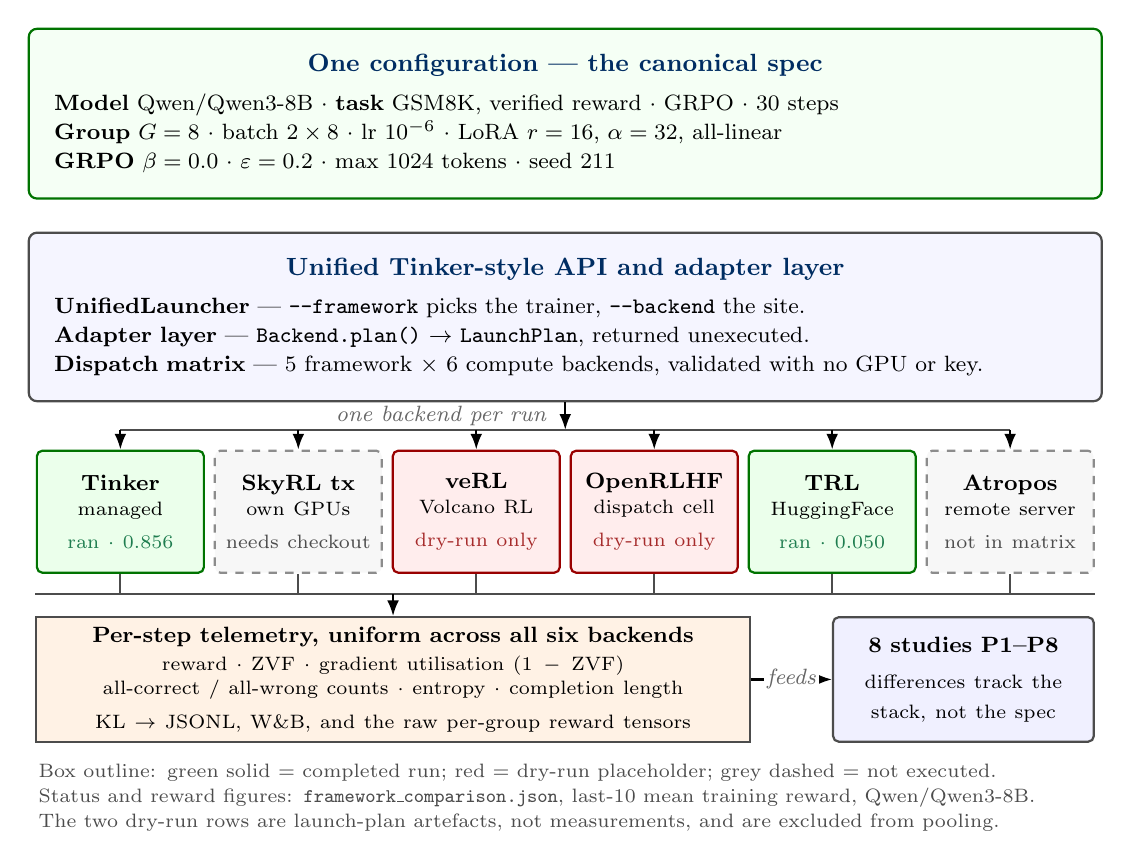
\begin{tikzpicture}[x=1cm,y=1cm,
  hdr/.style={font=\small\bfseries, text=pesblue, align=center, inner sep=1pt},
  card/.style={draw=green!45!black, thick, rounded corners=3pt, fill=green!4,
               inner sep=8pt, align=left},
  cardb/.style={draw=black!70, thick, rounded corners=3pt, fill=blue!4,
                inner sep=8pt, align=left},
  ctxt/.style={font=\footnotesize, align=left, text width=12.98cm, inner sep=1pt},
  bok/.style={oklbox, text width=1.91cm, minimum height=1.55cm, inner sep=3pt},
  bwarn/.style={warnbox, text width=1.91cm, minimum height=1.55cm, inner sep=3pt},
  bneu/.style={rectangle, rounded corners=2pt, draw=black!45, thick, dashed,
               fill=black!3, text width=1.91cm, minimum height=1.55cm,
               inner sep=3pt, align=center, font=\small},
  telb/.style={proc, text width=8.85cm, minimum height=1.58cm, inner sep=3pt},
  stdb/.style={blk, text width=3.10cm, minimum height=1.58cm, inner sep=3pt},
  busline/.style={draw=black!70, thick},
  phantom/.style={draw=none, fill=none, inner sep=0pt},
  note/.style={font=\scriptsize, align=left, text=black!70, inner sep=1pt},
]

% ===================== LAYER 1: the shared configuration =====================
\node[hdr, anchor=north] (c_h) at (0,0.35) {One configuration --- the canonical spec};
\node[ctxt, anchor=north] (c_b) at ([yshift=-4pt]c_h.south)
  {\textbf{Model} Qwen/Qwen3-8B $\cdot$ \textbf{task} GSM8K, verified reward
   $\cdot$ GRPO $\cdot$ 30 steps \\[1pt]
   \textbf{Group} $G=8$ $\cdot$ batch $2\times8$ $\cdot$ lr $10^{-6}$ $\cdot$
   LoRA $r=16$, $\alpha=32$, all-linear \\[1pt]
   \textbf{GRPO} $\beta=0.0$ $\cdot$ $\varepsilon=0.2$ $\cdot$ max 1024 tokens
   $\cdot$ seed 211};
\begin{scope}[on background layer]
  \node[card, fit=(c_h)(c_b)] (C1) {};
\end{scope}

% ===================== LAYER 2: unified API + adapter layer =====================
\node[hdr, anchor=north] (a_h) at ([yshift=-0.70cm]C1.south)
  {Unified Tinker-style API and adapter layer};
\node[ctxt, anchor=north] (a_b) at ([yshift=-4pt]a_h.south)
  {\textbf{UnifiedLauncher} --- \texttt{--framework} picks the trainer,
   \texttt{--backend} the site. \\[1pt]
   \textbf{Adapter layer} --- \texttt{Backend.plan()} $\to$ \texttt{LaunchPlan},
   returned unexecuted. \\[1pt]
   \textbf{Dispatch matrix} --- 5 framework $\times$ 6 compute backends,
   validated with no GPU or key.};
\begin{scope}[on background layer]
  \node[cardb, fit=(a_h)(a_b)] (C2) {};
\end{scope}

% ===================== LAYER 3: the six RL backends =====================
\coordinate (bus1) at ([yshift=-0.35cm]C2.south);
\coordinate (rowtop) at ([yshift=-0.25cm]bus1);
\draw[ar] (C2.south) -- (bus1);
\node[lbl, anchor=east] at ($(C2.south)!0.5!(bus1)+(-0.12,0)$) {one backend per run};
\draw[busline] (-5.65,0 |- bus1) -- (5.65,0 |- bus1);
\foreach \x in {-5.65,-3.39,-1.13,1.13,3.39,5.65}
  \draw[ar] (\x,0 |- bus1) -- (\x,0 |- rowtop);

\node[bok, anchor=north] (b1) at (-5.65,0 |- rowtop)
  {\footnotesize\textbf{Tinker}\\[1pt]\scriptsize managed\\[1pt]
   \scriptsize\textcolor{complete}{ran $\cdot$ 0.856}};
\node[bneu, anchor=north] (b2) at (-3.39,0 |- rowtop)
  {\footnotesize\textbf{SkyRL tx}\\[1pt]\scriptsize own GPUs\\[1pt]
   \scriptsize\textcolor{black!70}{needs checkout}};
\node[bwarn, anchor=north] (b3) at (-1.13,0 |- rowtop)
  {\footnotesize\textbf{veRL}\\[1pt]\scriptsize Volcano RL\\[1pt]
   \scriptsize\textcolor{blocked}{dry-run only}};
\node[bwarn, anchor=north] (b4) at (1.13,0 |- rowtop)
  {\footnotesize\textbf{OpenRLHF}\\[1pt]\scriptsize dispatch cell\\[1pt]
   \scriptsize\textcolor{blocked}{dry-run only}};
\node[bok, anchor=north] (b5) at (3.39,0 |- rowtop)
  {\footnotesize\textbf{TRL}\\[1pt]\scriptsize HuggingFace\\[1pt]
   \scriptsize\textcolor{complete}{ran $\cdot$ 0.050}};
\node[bneu, anchor=north] (b6) at (5.65,0 |- rowtop)
  {\footnotesize\textbf{Atropos}\\[1pt]\scriptsize remote server\\[1pt]
   \scriptsize\textcolor{black!70}{not in matrix}};
\node[phantom, fit=(b1)(b2)(b3)(b4)(b5)(b6)] (brow) {};

% ===================== LAYER 4: per-step telemetry =====================
\coordinate (bus2) at ([yshift=-0.25cm]brow.south);
\coordinate (bandtop) at ([yshift=-0.28cm]bus2);
\foreach \b in {b1,b2,b3,b4,b5,b6}
  \draw[busline] (\b.south) -- (\b.south |- bus2);
\draw[busline] (brow.west |- bus2) -- (brow.east |- bus2);

\node[telb, anchor=north west] (TEL) at (brow.west |- bandtop)
  {\footnotesize\textbf{Per-step telemetry, uniform across all six backends}\\[2pt]
   \scriptsize reward $\cdot$ ZVF $\cdot$ gradient utilisation ($1-\mathrm{ZVF}$)\\[1pt]
   \scriptsize all-correct / all-wrong counts $\cdot$ entropy $\cdot$ completion length\\[1pt]
   \scriptsize KL $\rightarrow$ JSONL, W\&B, and the raw per-group reward tensors};
\node[stdb, anchor=north west] (STD) at ([xshift=1.03cm]TEL.north east)
  {\footnotesize\textbf{8 studies P1--P8}\\[2pt]
   \scriptsize differences track the stack, not the spec};
\draw[ar] (TEL.east) -- (STD.west |- TEL.east);
\node[lbl, fill=white, inner sep=1pt] at ($(TEL.east)!0.5!(STD.west |- TEL.east)$) {feeds};
\draw[ar] (TEL.north |- bus2) -- (TEL.north);

% ===================== SOURCE AND LEGEND NOTE =====================
\node[phantom, fit=(TEL)(STD)] (band) {};
\coordinate (notetop) at ([yshift=-0.22cm]band.south);
\node[note, anchor=north west, text width=13.40cm] at (brow.west |- notetop)
  {Box outline: green solid = completed run; red = dry-run placeholder; grey dashed = not executed.\\[1pt]
   Status and reward figures: \texttt{framework\_comparison.json}, last-10 mean training reward, Qwen/Qwen3-8B.\\[1pt]
   The two dry-run rows are launch-plan artefacts, not measurements, and are excluded from pooling.};

\end{tikzpicture}
\end{document}
